\nonstopmode

\documentclass[letterpaper,12pt,titlepage]{article}
\usepackage{amsthm,amssymb,mathtools}
\mathtoolsset{showonlyrefs}
\usepackage{bm}
\usepackage[margin=1in]{geometry}
\usepackage{booktabs}
\usepackage{enumitem}
\usepackage{framed}
\usepackage{tikz}
\usetikzlibrary{shapes,arrows,positioning,patterns,calc}
\usepackage{pgfplots}
\pgfplotsset{compat=1.9}
\usepackage{listings}
\usepackage[numbered,framed]{mcode}

\usepackage{fancyhdr}
\pagestyle{fancy}
\fancyhead{}
\fancyfoot{}
\fancyfoot[L]{K.\ Okkelberg}
\fancyfoot[R]{\thepage}
\renewcommand{\headrulewidth}{0pt}
\renewcommand{\footrulewidth}{0.5pt}

\newcommand*\dif{\mathop{}\!\mathrm{d}}
\newcommand{\trans}{^\text{T}}
\newcommand{\herm}{^\text{H}}
\DeclareMathOperator{\E}{E}
\DeclareMathOperator{\trace}{trace}
\DeclareMathOperator{\sign}{sign}
\let\Pr\relax
\DeclareMathOperator{\Pr}{P}
\newcommand*\pder[2]{\frac{\partial #1}{\partial #2}}
\newcommand*\R{\mathbb{R}}

\tikzstyle{line} = [draw,>=latex]
\tikzstyle{dot} = [circle,fill=black,inner sep=0pt,minimum size=4pt]

\begin{document}

\title{ECE 6553: Homework \#1}
\author{Klaus Okkelberg}
\date{January 26, 2017}
\maketitle

\setlist{listparindent=\parindent}

\begin{enumerate}[leftmargin=0pt]

\item \begin{enumerate}
  \item Consider vectors $\epsilon v\in\R^m$, $\epsilon\in\R$, $\Vert v\Vert=1$. Notice that $\epsilon$ is the magnitude and $v$ is the direction of the vector. The size of the growth of $g(u)$ in the direction of $\epsilon v$ is given by
    \begin{align}
      g(u+\epsilon v) - g(u) &= g(u) + \epsilon\pder{g}{u}(u)v + o(\epsilon) - g(u) \\
                             &= \epsilon\pder{g}{u}(u)v + o(\epsilon) \\
                             &= \epsilon \pder{g\trans}{u}(u) \cdot v + o(\epsilon) \\
                             &= \epsilon \nabla g(u) \cdot v + o(\epsilon) \\
                             &= \epsilon \Vert\nabla g(u)\Vert \, \Vert v\Vert \cos\theta + o(\epsilon) \\
                             &= \epsilon \Vert\nabla g(u)\Vert \cos\theta + o(\epsilon),
    \end{align}
    where $\theta$ is the angle between $\nabla g(u)$ and $v$. For a given $\epsilon$, we can see that the amount of increase is maximized when $\theta=0$, i.e.\ $v$ points along $\nabla g(u)$. Therefore, $g$ grows the most in the direction of $\nabla g(u)$. \qed
    
  %\item The directional derivative of $g:\R^m\to\R$ at $u\in\R^m$ along $v\in\R^m$ is given by
  %  \begin{align}
  %    \delta g(u;v) &= \lim_{h\to0} \frac{g(u+hv)-g(u)}{h} \\
  %                  &= \lim_{h\to0} \frac{g(u)+h\pder{g}{u}(u)v-g(u)+o(h)}{h} \\
  %                  &= \pder{g}{u}(u) v \\
  %                  &= pder{g\trans}{u}(u) \cdot v \\
  %                  &= \nabla g(u) \cdot v \\
  %                  &= \Vert\nabla g(u)\Vert \Vert v\Vert \cos \theta,
  %  \end{align}
  %  where $\theta$ is the angle between $\nabla g(u)$ and $v$. This directional derivative indicates how much $g$ grows at the point $u$ in the direction of $v$. Notice that it is maximized when $\nabla g(u)$ and $v$ are aligned, i.e.\ $g$ grows the most along $v=\nabla g(u)$.

  \item Let $u=r(t)$, $t\in\R$, be the curve that satisfies the constraint $h(u)=0$, i.e.\ $h(r(t))=0$ $\forall t$. Since the constraint condition is constant, taking the derivative of the constraint gives
    \begin{align}
      \frac{\dif}{\dif t} h(r(t)) &= \pder{h(r(t))}{r(t)} \frac{\dif r(t)}{\dif t} \\
                                  &= \pder{h(u)}{u} r'(t) \\
                                  &= \nabla h(u) \cdot r'(t) = 0
    \end{align}
    Notice that the derivative of the curve $r'(t)$ is the tangent plane to the constraint set at $u$. Since the dot product of the gradient and $r'(t)$ is 0, the gradient $\nabla g(u)$ is orthogonal to the tangent plane to the constraint set at $u$. \qed
  \end{enumerate}

\item The Lagrangian is
  \[ L = (u_1-2)^2 + 2(u_2-1)^2 + \lambda_1(u_1+4u_2-3) + \lambda_2(u_2-u_1) \]
  The FONCs are
  \begin{align}
    \pder{L}{u_1} = 2(u_1-2) + \lambda_1 - \lambda_2 &= 0 \\
    \pder{L}{u_2} = 4(u_2-1) + 4\lambda_1 + \lambda_2 &= 0\\
    \lambda_1(u_1+4u_2-3) &= 0 \\
    \lambda_2(u_2-u_1) &= 0 \\
    u_1+4u_2-3 &\le 0 \\
    u_2-u_1 &\le 0 \\
    \lambda_1 &\ge 0 \\
    \lambda_2 &\ge 0
  \end{align}

  Consider the following combinations in which the constraints can be active/inactive:
  \begin{enumerate}
  \item $\lambda_1=\lambda_2=0$
    \[ \begin{cases}
        2(u_1-2) = 0 \\
        4(u_2-1) = 0
      \end{cases} \Longrightarrow
      \begin{cases}
        u_1 = 2 \\
        u_2 = 1
      \end{cases} \]
    Since $u_1+4u_2 \nleq 3$, this solution is not feasible.
  \item $u_1+4u_2-3 = 0$, $\lambda_2=0$
    \[ \begin{cases}
        2(u_1-2) + \lambda_1 = 0 \\
        4(u_2-1) + 4\lambda_1 = 0 \\
        u_1 + 4u_2 = 3
      \end{cases} \Longrightarrow
      \begin{bmatrix} u_1 \\ u_2 \\ \lambda_1 \end{bmatrix} =
      \begin{bmatrix}
        2 & 0 & 1 \\
        0 & 4 & 4 \\
        1 & 4 & 0
      \end{bmatrix}^{-1}
      \begin{bmatrix}
        4 \\ 4 \\ 3
      \end{bmatrix} =
      \begin{bmatrix}
        5/3 \\ 1/3 \\ 2/3
      \end{bmatrix}
    \]
    We can verify that the constraints hold:
    \begin{align}
      u_1 + 4u_2 &\le 3 \\
      u_1 &\ge u_2
    \end{align}
    Therefore, $u_1=5/3$, $u_2=1/3$ is a local minimizer.
  \item $\lambda_1=0$, $u_1=u_2$
    \[ \begin{cases}
        2(u_1-2) - \lambda_2 = 0 \\
        4(u_2-1) + \lambda_2 = 0 \\
        u_1 = u_2
      \end{cases} \Longrightarrow
      \begin{bmatrix}
        u_1 \\ u_2 \\ \lambda_2
      \end{bmatrix} =
      \begin{bmatrix}
        2 & 0 & -1 \\
        0 & 4 & 1 \\
        1 & -1 & 0
      \end{bmatrix}^{-1}
      \begin{bmatrix}
        4 \\ 4 \\ 0
      \end{bmatrix} =
      \begin{bmatrix}
        4/3 \\ 4/3 \\ -4/3
      \end{bmatrix}
    \]
    Since $\lambda_2<0$, this solution is not feasible.
  \item $u_1+4u_2-3=0$, $u_1=u_2$
    \[ \begin{cases}
        2(u_1-2) + \lambda_1 - \lambda_2 = 0 \\
        4(u_2-1) + 4\lambda_1 + \lambda_2 = 0 \\
        u_1 + 4u_2 = 3 \\
        u_1 = u_2
      \end{cases} \Longrightarrow
      \begin{bmatrix}
        u_1 \\ u_2 \\ \lambda_1 \\ \lambda_2
      \end{bmatrix} =
      \begin{bmatrix}
        2 & 0 & 1 & -1 \\
        0 & 4 & 4 & 1 \\
        1 & 4 & 0 & 0 \\
        1 & -1 & 0 & 0
      \end{bmatrix}^{-1}
      \begin{bmatrix}
        4 \\ 4 \\ 3 \\ 0
      \end{bmatrix} =
      \begin{bmatrix}
        3/5 \\ 3/5 \\ 22/25 \\ -48/25
      \end{bmatrix}
    \]
    Since $\lambda_2<0$, this solution is not feasible.

    Since the optimization problem only has one feasible solution, the global minimum is given by
    \begin{align}
      u^*_1 &= 5/3 \\
      u^*_2 &= 1/3
    \end{align}
  \end{enumerate}

\item \begin{enumerate}
  \item The minimization problem is
    \begin{gather}
      \min \alpha u_1^2 + \beta u_2^2 \\
      \text{s.t. } u_1 + u_2 = q
    \end{gather}
    The Lagrangian is
    \[ L = \alpha u_1^2 + \beta u_2^2 + \lambda(u_1+u_2-q) \]
    The FONCs are
    \begin{align}
      \pder{L}{u_1} = 2\alpha u_1 + \lambda &= 0 \\
      \pder{L}{u_2} = 2\beta u_2 + \lambda &= 0 \\
      \pder{L}{\lambda} = u_1+u_2-q &= 0
    \end{align}
    From the first two conditions, $\alpha u_1 = \beta u_2$. Substituting this into the third condition gives
    \begin{align}
      u_1 &= \frac{\beta}{\alpha+\beta} q \\
      u_2 &= \frac{\alpha}{\alpha+\beta} q
    \end{align}
  \item It is clear that the highest cost is achieved by only shipping through the more expensive option, i.e.
    \[
      \begin{cases}
        \max \alpha u_1^2 + \beta u_2^2 \\
        \text{s.t. } u_1 + u_2 = q
      \end{cases}
      \Longrightarrow
      \begin{cases}
        u^*_i = q, & i = \arg\max(\alpha,\beta) \\
        u^*_j = 0, & j = \arg\min(\alpha,\beta)
      \end{cases}
    \]
    This gives a total cost of $\max(\alpha,\beta)\cdot q^2$. The cost of the minimizers from the previous part is
    \[ \alpha \left(\frac{\beta}{\alpha+\beta} q\right)^2 + \beta \left(\frac{\alpha}{\alpha+\beta} q\right)^2 = \frac{\alpha\beta}{\alpha+\beta} q^2 < \min(\alpha,\beta)\cdot q^2 \le \max(\alpha,\beta)\cdot q^2 \]
    Therefore, the combination found in the previous part is not the worst combination and must be the best combination instead.
  \end{enumerate}

\item By convexity of $g$, for all $u\in\R^m$ and $\alpha\in[0,1]$,
  \begin{gather}
    g(\alpha u + (1-\alpha)u^*) \le \alpha g(u) + (1-\alpha)g(u^*) \\
    g(\alpha u + (1-\alpha)u^*) \le g(u^*) + \alpha (g(u)-g(u^*)) \\
    g(u)-g(u^*) \ge \frac{g(\alpha u + (1-\alpha)u^*) - g(u^*)}{\alpha}
  \end{gather}
  Using L'H\^opital's rule to take the limit as $\alpha\to0$,
  \begin{align}
    g(u)-g(u^*) &\ge \lim_{\alpha\to0} \frac{g(\alpha u + (1-\alpha)u^*) - g(u^*)}{\alpha} \\
                &= \left[ \frac{\dif}{\dif\alpha} \Big\{ g(\alpha u + (1-\alpha)u^*) - g(u^*) \Big\} \right]_{\alpha=0} \\
                &= \pder{g}{u}(u^*) \left[ \frac{\dif}{\dif\alpha} (\alpha u + (1-\alpha)u^*) \right]_{\alpha=0} \\
                &= \pder{g}{u}(u^*) (u - u^*) = 0\cdot(u-u^*) = 0
  \end{align}
  Since $g(u)-g(u^*)\ge0$, or $g(u^*)\le g(u)$ $\forall u\in\R^m$, $u^*$ is the global minimum to $g$.

%\item Assume that $u^*$ is not the global minimum to $g$. Therefore, there exists $u_0\ne u^*$ such that $g(u_0)<g(u^*)$. By convexity of $g$, for $0<\alpha\le 1$,
%  \[
%    g(\alpha u_0 + (1-\alpha)u^*) \le \alpha g(u_0) + (1-\alpha)g(u^*) < \alpha g(u^*) + (1-\alpha)g(u^*) = g(u^*)
%  \]
%  Since 

\item The minimization problem is
  \[ \gamma_k^{\min} = \arg\min_\gamma g(u_k+\gamma d_k) \]
  The first and second derivatives of $g(u)$ are
  \begin{align}
    \pder{g}{u}(u) &= u\trans Q + b\trans \\
    \pder{^2 g}{u^2}(u) &= Q
  \end{align}
  From the Hessian, the cost is convex and a stationary point is a global minimum. Therefore, we solve the problem by taking the derivative of the cost at $k$:
  \begin{align}
    \frac{\dif}{\dif\gamma} g(u_k+\gamma d_k) &= \pder{g}{u}(u_k+\gamma d_k) \frac{\dif}{\dif\gamma}(u_k+\gamma d_k) \\
                                              &= \Big[(u_k+\gamma d_k)\trans Q + b\trans\Big] d_k \\
                                              &= \Big(u_k\trans Q + \gamma d_k\trans Q + b\trans\Big) d_k = 0 \\
    \gamma &= \frac{-(u_k\trans Q + b\trans) d_k}{d_k\trans Q d_k} \\
    \shortintertext{Using $d_k=-(u_k\trans Q+b\trans)\trans=-(Qu_k+b)$,}
    \gamma_k^{\min} &= \frac{d_k\trans d_k}{d_k\trans Q d_k}
  \end{align}
  \clearpage
\item \begin{enumerate}
  \item \mbox{}

      \begin{figure}[h!]
        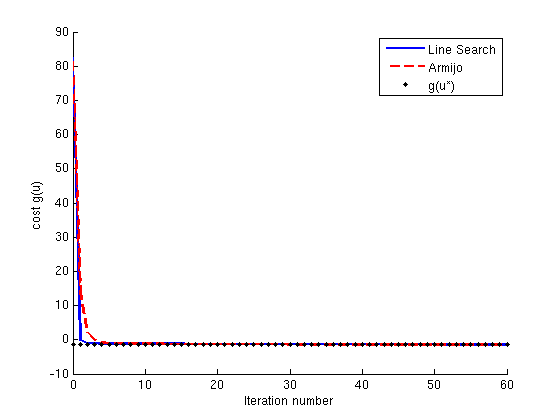
\includegraphics[width=0.76\textwidth]{hw1p6a}
        \caption{Cost of line search and Armijo vs iteration.}
      \end{figure}
      \begin{figure}[h!]
        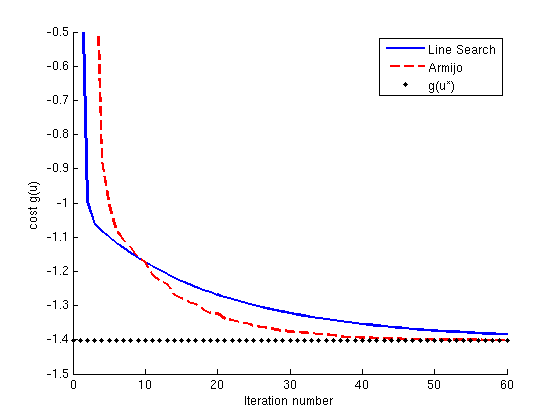
\includegraphics[width=0.76\textwidth]{hw1p6a_detail}
        \caption{Detailed view of cost of line search and Armijo vs iteration.}
      \end{figure}
    
    \clearpage
    \lstinputlisting{hw1p6.m}

  \item While line search is initially faster, Armijo is faster overall.

    This is not always the case. For example, for $u_0$ such that $-\nabla g(u_0)$ is in the direction of the minimizer $u^*$, line search would reach $u^*$ in one iteration, whereas the Armijo method would need more than one iteration with most $\alpha$ and $\beta$.

    Even if one method is always better than the other (in terms of iteration count), it likely has other costs like computation or memory. It is true that Armijo converges faster, but each iteration of the method is much more costly computation-wise than the line search method.
    
  \end{enumerate}
  
\end{enumerate}

\end{document}
